\documentclass[10pt,a4paper]{article}

\usepackage[T1]{fontenc}
\usepackage[margin=1.5cm]{geometry}
\usepackage{amsmath,amssymb}
\usepackage{booktabs}
\usepackage{array}
\usepackage{enumitem}
\usepackage{graphicx}
\usepackage{tikz}
\usetikzlibrary{arrows.meta,positioning,patterns}
\usepackage[hidelinks]{hyperref}
\usepackage{titlesec}
\usepackage{parskip}

\setlist{itemsep=0pt,topsep=1pt,parsep=0pt,leftmargin=1.1em}
\titleformat{\section}{\bfseries\large}{\thesection.}{0.4em}{}
\titlespacing*{\section}{0pt}{5pt}{2pt}
\setlength{\parskip}{2.5pt}
\renewcommand{\arraystretch}{1.12}
\pagestyle{empty}

\begin{document}

\begin{center}
{\large\bfseries Midterm Report: Short Explanation}\\[1pt]
{\small Change-Characteristic-Aware Window Selection for Unsupervised Concept Drift Detection in Real-Time Text Streams}
\end{center}
\vspace{-4pt}

\section{The problem}
Text such as news, posts and reviews keeps arriving. Over time the topics and words change. This is called \textbf{concept drift}. A model trained on old text then becomes less accurate, so a real-time system must notice the change quickly. Most detectors need the true label of every document, but for text the labels come late or never. So we need a detector that works \textbf{without labels}. Many detectors compare a \textbf{window} of recent data with older data. A short window reacts fast but gives false alarms. A long window is steady but slow. The best size depends on the type of drift.

\section{Base paper and research gap}
Our base paper is \textbf{ADWIN-U} (Assis and Souza, \emph{Knowledge and Information Systems}, 2025). It builds on \textbf{ADWIN} (Bifet and Gavald\`a, 2007). ADWIN keeps a window $W$ and splits it into an older part $W_1$ and a newer part $W_2$. If the averages of the two parts differ by more than a threshold $\varepsilon$, it says a change happened and \textbf{drops all of $W_1$}:
\[
|\hat\mu_{W_1}-\hat\mu_{W_2}|\ \ge\ \varepsilon .
\]
The threshold $\varepsilon$ is the size of a gap that is too big to be luck. It depends on a confidence level $\delta$: a smaller $\delta$ means a bigger $\varepsilon$ and a stricter test. ADWIN-U removes the need for labels by watching a simple number from each example (skewness or kurtosis) instead of the error.

\textbf{Gap.} (1) ADWIN-U uses one fixed $\delta$ for every drift. (2) It always cuts the whole old part, whether the change is strong or weak, short or long. (3) It was tested only on numeric sensor-type data, never on text.

\section{Our contribution}
We add a small rule that decides \emph{how much} of the window to cut. It uses two thresholds, a strict $\varepsilon_s$ (``sure'') and a relaxed $\varepsilon_w$ (``maybe''), where $\varepsilon_s>\varepsilon_w$. Let $g=\hat\mu_{W_1}-\hat\mu_{W_2}$ be the gap with its sign.
\begin{itemize}
  \item \textbf{Strong gap} ($|g|\ge\varepsilon_s$): \textbf{full cut}, same as ADWIN-U.
  \item \textbf{Weak gap} ($\varepsilon_w\le|g|<\varepsilon_s$): \textbf{hold}. Do not cut, raise a warning and count in $c$ the checks in a row with the same sign. If the gap vanishes or the sign flips, release the hold.
  \item \textbf{Hold lasts $k$ checks:} \textbf{graded cut}. Drop only the oldest share $\rho=\min(1,|g|/\varepsilon_s)$ of $W_1$. A bigger gap drops more.
\end{itemize}
\textbf{Example.} If $\varepsilon_s=0.10$ and a weak gap stays at $0.05$ for $k$ checks, then $\rho=0.5$ and we drop the oldest half of $W_1$ (an illustration, not a result).

\textbf{How we differ from ADWIN-U.} It has one choice (full cut), we have three (full cut, hold, graded cut). It has one $\delta$, we have two. It was tested on numbers, we test on text. ADWIN-U is a special case of ours: if $\delta_w=\delta_s$, the weak zone is empty and the two methods are the same. We do \emph{not} claim to invent adaptive windows or label-free monitoring. Our contribution is the cut rule and its test on text.

\begin{center}
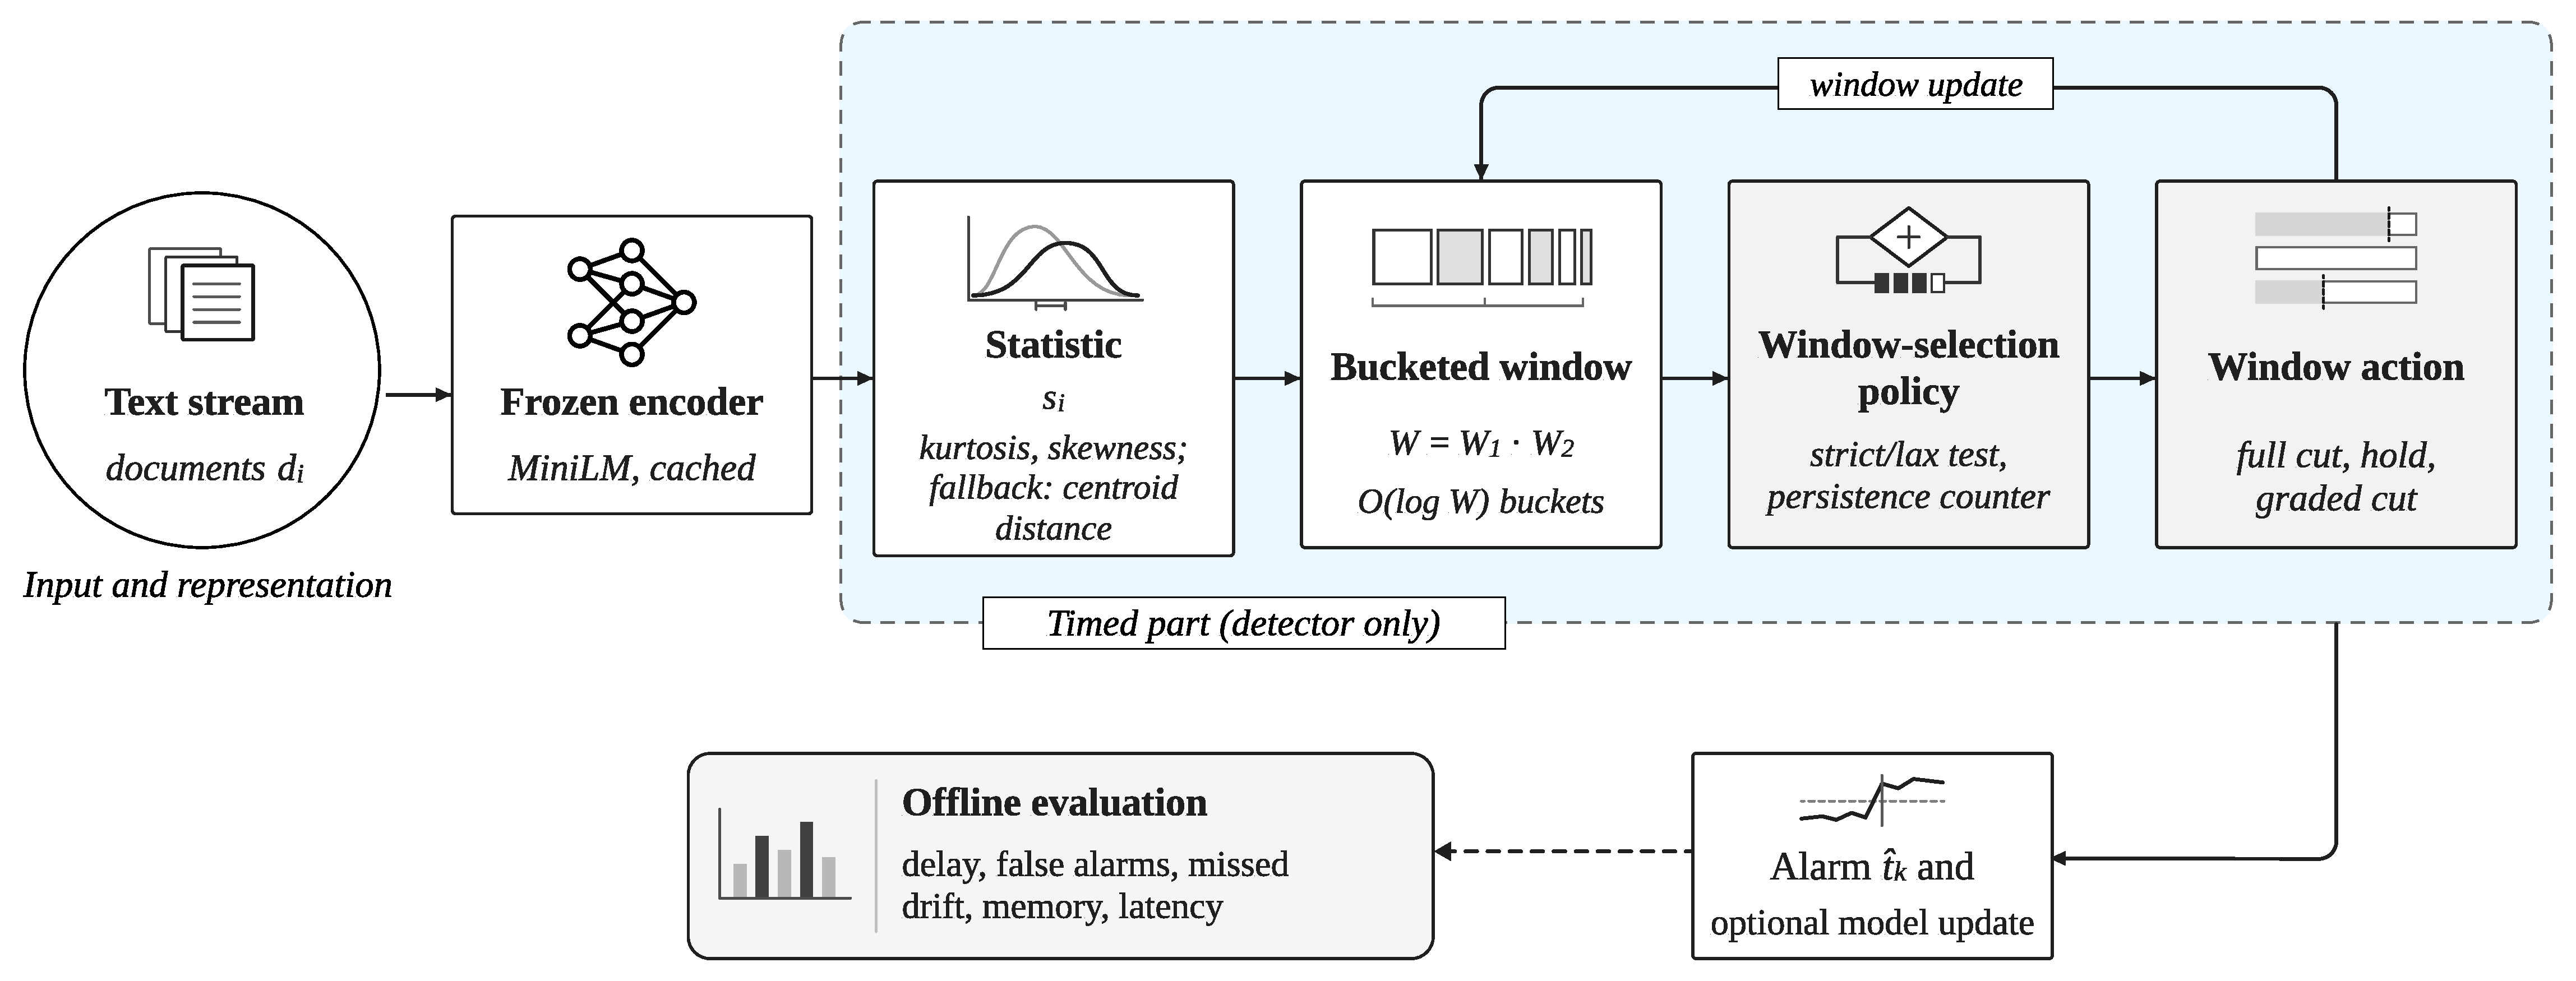
\includegraphics[width=0.9\linewidth]{figures/pipeline.pdf}\\[2pt]
{\small\textbf{Figure 1 (pipeline).} Text goes through a frozen Sentence-BERT encoder (embeddings are saved, so timing covers only the detector), then one number per embedding, then ADWIN's window, then our policy (shaded), which gives the action and the alarm.}
\end{center}

\section{Methodology in simple steps}
(1) The detector sees only the embedding of each document, never the label. (2) A frozen Sentence-BERT model turns each document into 384 numbers. (3) We compute one statistic per embedding, such as kurtosis or skewness (cosine distance to the window centre is the backup). (4) The statistic goes into ADWIN's bucketed window, which needs only $O(\log W)$ time and memory. (5) Our policy picks full cut, hold or graded cut (Figures 2 and 3).

\begin{center}
\begin{minipage}[c]{0.52\linewidth}
\centering
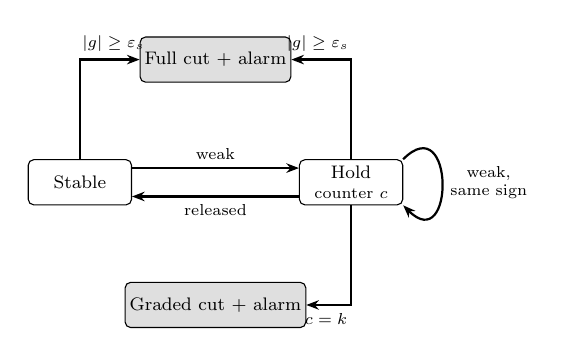
\begin{tikzpicture}[scale=0.82, transform shape,
  st/.style={draw, rounded corners=2pt, align=center, minimum height=7mm, minimum width=1.6cm, inner sep=2pt, font=\footnotesize, fill=white},
  ac/.style={draw, rounded corners=2pt, align=center, minimum height=7mm, inner sep=2pt, font=\footnotesize, fill=gray!25},
  arr/.style={-{Stealth[length=1.6mm]}, thick},
  lab/.style={font=\scriptsize, align=center}
]
\node[st] (stable) at (0,0) {Stable};
\node[st] (hold) at (4.2,0) {Hold\\[-1pt]{\scriptsize counter $c$}};
\node[ac] (full) at (2.1,1.9) {Full cut + alarm};
\node[ac] (grad) at (2.1,-1.9) {Graded cut + alarm};
\draw[arr] (stable.north) |- node[lab, pos=0.78, above] {$|g|\ge\varepsilon_s$} (full.west);
\draw[arr] (hold.north) |- node[lab, pos=0.78, above] {$|g|\ge\varepsilon_s$} (full.east);
\draw[arr] ([yshift=2.2mm]stable.east) -- node[lab, above] {weak} ([yshift=2.2mm]hold.west);
\draw[arr] ([yshift=-2.2mm]hold.west) -- node[lab, below] {released} ([yshift=-2.2mm]stable.east);
\draw[arr] (hold.south) |- node[lab, pos=0.78, below] {$c=k$} (grad.east);
\draw[arr] (hold.north east) .. controls +(0.8,0.8) and +(0.8,-0.8) .. node[lab, right, pos=0.5] {weak,\\same sign} (hold.south east);
\end{tikzpicture}

{\small\textbf{Figure 2.} Rules of the policy.}
\end{minipage}\hfill
\begin{minipage}[c]{0.46\linewidth}
\centering
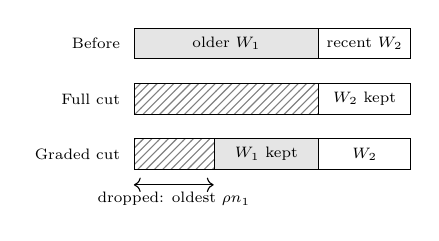
\begin{tikzpicture}[scale=0.78, transform shape,
  seg/.style={draw, minimum height=5mm, inner sep=0pt, font=\scriptsize},
  lab/.style={font=\scriptsize, anchor=east}
]
\def\a{3.0} \def\b{1.5} \def\d{1.3} \pgfmathsetmacro{\r}{\a-\d}
\node[lab] at (0,0) {Before};
\node[seg, minimum width=\a cm, fill=gray!20, anchor=west] at (0.1,0) {older $W_1$};
\node[seg, minimum width=\b cm, fill=white, anchor=west] at (\a+0.1,0) {recent $W_2$};
\node[lab] at (0,-0.9) {Full cut};
\node[seg, minimum width=\a cm, pattern=north east lines, pattern color=black!50, anchor=west] at (0.1,-0.9) {};
\node[seg, minimum width=\b cm, fill=white, anchor=west] at (\a+0.1,-0.9) {$W_2$ kept};
\node[lab] at (0,-1.8) {Graded cut};
\node[seg, minimum width=\d cm, pattern=north east lines, pattern color=black!50, anchor=west] at (0.1,-1.8) {};
\node[seg, minimum width=\r cm, fill=gray!20, anchor=west] at (\d+0.1,-1.8) {$W_1$ kept};
\node[seg, minimum width=\b cm, fill=white, anchor=west] at (\a+0.1,-1.8) {$W_2$};
\draw[<->, thin] (0.1,-2.3) -- node[font=\scriptsize, below] {dropped: oldest $\rho n_1$} (\d+0.1,-2.3);
\end{tikzpicture}

{\small\textbf{Figure 3.} Full cut and graded cut (striped = dropped).}
\end{minipage}
\end{center}

\textbf{Why the figures.} Figure~1 shows the whole system and where our new part fits. Figure~2 shows that every case has a defined action. Figure~3 shows the main difference from ADWIN-U: it always does the full cut, while ours can keep useful older data when the change is small.

\section{Evaluation plan}
\textbf{Datasets.} \emph{AG News}: we change the topic mix to make abrupt, gradual and recurring drift (known). \emph{20 Newsgroups}: swapping far-apart groups gives strong drift and swapping sibling groups gives subtle drift (known). \emph{Amazon reviews}: a real stream in time order (drift unknown, so we use proxies such as alarm rate and downstream accuracy).

\textbf{Baselines.} ADWIN-U, ADWIN with many $\delta$ values, a warning/alarm variant, KSWIN-style and D3-style detectors.

\textbf{Metrics.} Time to detection, false alarms per 1,000 items, missed-drift rate, window length, latency, peak memory and throughput (BAR as extra). All methods are set to the \emph{same false-alarm rate} first, then compared with Friedman and Nemenyi tests. Ablations remove parts of our method to see what helps.

\section{Big data characteristics}
\noindent\begin{tabular}{@{}>{\bfseries}p{1.6cm}p{7.2cm}p{7.2cm}@{}}
\toprule
 & Why it applies & How we handle it \\
\midrule
Velocity & Documents arrive all the time, one pass only. & Compact window, almost constant time per item. We measure latency and throughput. \\
Variety & Text is unstructured, with many topics and styles. & Sentence embeddings, so one detector fits news, posts and reviews. \\
Veracity & Labels are missing and true drift points are unknown. & No labels. The hold state avoids acting on one weak signal. \\
\bottomrule
\end{tabular}\par\smallskip
We do not claim Volume. Our variety means topics and styles, not many data types.

\section{Status and honest limits}
This midterm report gives the \textbf{idea and the plan}. The experiments are not done yet, so we say ``expected'' and not ``proved''. Two risks: skewness or kurtosis may not react to topic change (we test it first and have a backup), and the relaxed test with persistence has no formal false-alarm guarantee (so we measure false alarms on streams with no drift). \textbf{Next:} build the text streams, implement the policy on ADWIN-U, run all baselines and report the results.

\end{document}
